\chapter{Grundlagen}\label{ch:grundl}



\sectionDM{Spielprinzip von Josie - A Jelly's Journey}
\gamename  erinnert an eine erweiterte Version des Spieleklassikers Super Mario World.
In der Theorie sollte es mehrere Spielabschnitte geben, jedoch wurde aus zeitlichen Gründen nur ein Abschnitt implementiert. Ein Spielabschnitt besteht aus drei Jump and Run Levels und einem Boss Kampf Level. 

\paragraph{Jump and Run Level:}
Der Spieler versucht ohne Zeiteinschränkung das Level abzuschließen und dabei so viele Münzen wie möglich zu sammeln. Bei einem perfekten Lauf \textbf{kann} man alle Münzen einsammeln, einige davon sind allerding so plaziert dass sie nur schwer zu erreichen sind.
Dem Spieler stehen die Steuerungsfunktionen "'Stoppen"', "'Schrumpfen"' und "'Springen"' zur Verfügung. 
Dass Josie von selbst in einer festgelegten Geschwindigkeit läuft, führt zu einer gewissen Schwierigkeit des Spiels und macht Steuerungsfunktionen für "'Links"' und "'Rechts"' überflüssig.

\paragraph{Boss Level:}



\sectionTL{Framework}\label{sec:2_Framework}
Als die grobe Idee für das Spiel feststand, mussten wir uns für eine GameEngine entscheiden. Zur Auswahl standen unter anderem die AndEngine, Unity und Cocos2d-x. Nach ausreichender Recherche über die Funktionalitäten der verschiedenen Engines haben wir uns einstimmig für Cocos2d-x entschieden. Cocos2d-x untestützt drei Programmiersprachen, C++, JavaSkript und Lua. Hier haben wir C++ gewählt, da wir im laufe unseres Studiums eine Vorlesung über C++ gehört haben.
Die nächste Herausforderung war die Einrichtung von Cocos2d-x. Da wir drei verschiedene Betriebssysteme(Win8, MacOSX, Ubuntu) benutzen, hatten wir geringe Kompatibilitätsprobleme.
Um Cocos2d-x einzurichten, werden folgende Pakete benötigt:

\begin{itemize}
\item Cocos2d-x Link - http://www.cocos2d-x.org/download
\item Android SDK - http://developer.android.com/sdk/index.html
\item Android NDK - http://androids.zone/android-ndk/#.VBLHNPldWXY
\item Apache Ant - http://ant.apache.org/bindownload.cgi
\item Python - https://www.python.org/downloads/
\item Eclipse – https://eclipse.org/downloads/
\end{itemize}

Nachdem die Pakete heruntergeladen und ausgepackt sind, verschiebt man diese in den selben Ordner. Apache Ant und Python müssen installiert werden. Bei Python muss darauf geachtet werden das es sich um Version 2.x handelt. Unter Ubuntu muss Python nicht installiert werden, da dies schon in den Paketquellen vorhanden ist. 
Hat man die zwei Programme installiert öffnet man den Cocos2d-x Ordner und startet die setup.py Datei (über das Terminal). Daraufhin öffnet sich ein Terminalfenster in dem die Umgebungsvariablen angepasst werden, dies bedeutet man wird nach den Pfaden von der Android SDK/NDK, Apache Ant und Python gefragt. Entweder man gibt diese per Hand ein oder zieht die jeweiligen Ordner in das Terminalfenster. 



\sectionTL{IDE und Plugins}\label{sec:2_IDE}

Nachdem die Umgebungsvariablen eingetragen sind, muss das Android Developer Tool Plugin für Eclipse installiert werden. Hat man das erledigt öffnet man den im Plugin enthaltenen Android SDK-Manager und lädt sich hier nochmal die passende API herunter. In unserem Fall war das die API für Androidversion 4.4.2(API 19). 
Ist dieser Schritt geschafft, wird es Zeit das erste Projekt zu erstellen.
Hierzu öffnet man einen Terminal und wechselt in das Verzeichnis in dem auch der Cocos2d-x Ordner liegt. Hier gibt man folgenden Befehl ein:
	
\begin{lstlisting}[style=singleline]
	$cocos new MyGame -p com.MyCompany.MyGame -l cpp -d ~/MyCompany
\end{lstlisting}
		
\begin{itemize}
\item MyGame gibt den Namen des Projekts an
\item com.MyCompany.MyGame ist der Paketname für Android
\item cpp steht für die Programmiersprache. cpp für C++ und lua für Lua
\item ~/MyCompany gibt das Verzeichnis an in dem das Projekt gespeichert wird 
\end{itemize}

Der somit erstelle Ordner wird ins Git-Repository hochgeladen. 
Nun öffnet man wieder Eclipse und importiert das Git-Repository sowie die Cocos2d-x Bibliotheken. 

	Git-Repository: Eclipse → File → Import... → Git → 'Projects from Git'

Hier wählt man das vorher erstellte Projekt im Git-Repository aus.

	Cocos2d-x Bibliotheken: Eclipse → Import... → Android → 'Existing Android Code into 	Workspace'

Hier dirigiert man in das Verzeichnis in dem der Cocos2d-x Ordner liegt und wählt diesen komplett aus. Im nachfolgenden Fenster wählt man alle vorgeschlagenen Punkte ab bis auf libcocos2dx Nachdem beide 'Projekte' importiert wurden, wählt man sein Projekt aus dem Git-Repository aus und wechselt in die Einstellungen. Unter dem Reiter 'Android' ist darauf zu achten, dass als Library das Projekt libcocos2dx ausgewählt ist. Ist es nicht in der Liste enthalten, fügt man es mit 'Add' hinzu. 

Es ist darauf zu achten, dass sich alle Ordner inkl. dem Git-Repository in einem Ordner befinden.

Zu guter Letzt, öffnet man die AndroidManifest.xml in Eclipse aus und ändert hier den Wert auf die Entsprechende API.
\begin{lstlisting}[style=singleline]
	<uses-sdk android:minSdkVersion="19"
			  android:targetSdkVersion="19"/>
\end{lstlisting}
	

Nun kann man anfangen zu arbeiten! 



\sectionTL{Szenenprinzip}\label{sec:2_Szenenprinzip}
Eine Szene ist im Grunde genommen nichts anderes als ein Container, welcher  Sprites, Labels, Nodes und andere Objekte beinhaltet die ein Spiel benötigt. Eine Szene ist für die laufende Spiellogik und Darstellung des Inhaltes auf einer 'per-frame basis' verantwortlich. Es wird mindestens eine Szene benötigt damit man das Spiel starten kann. Man kann beliebig viele Szenen-Objekte in einem Spiel verwenden und leicht zwischen diesen überleiten. Der Vorteil von Szenen liegt darin, dass man nicht jedes Objekt einzeln laden muss. An eine Szene lassen sich diverse Sprites, Labels und Nodes mit der von Cocos2d-x gegebenen Funktion addChild() anhängen(siehe Abbildung \ref{fig:szenengraph}). Sobald das Szenen-Objekt geladen wird, werden die angefügten Kinder mitgeladen. Dies spart Zeit und entlastet den Speicher.

\begin{figure}[H]
  \centering
  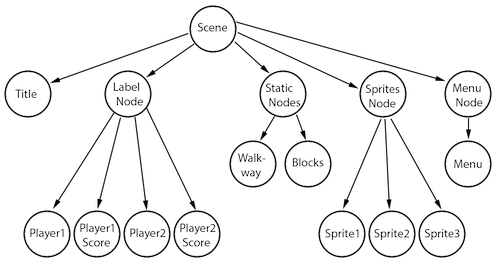
\includegraphics[width=12cm]{resources/scenegraph}
  \caption{Szenengraph}
  \label{fig:szenengraph} 
\end{figure}


\subsection{Szenenfunktionen von cocos2d}

Cocos bietet Funktionen an um Szenen zu erstellen und zwischen diesen zu wechseln. Um einen Szenenwechsel durchzufüren, muss zuerst eine Szene erstellt werden.

\begin{lstlisting}[style=singleline]
	Szene* Cutscene = Szene::create();
\end{lstlisting}


Dies erstellt ein Objekt des Typ Szene mit dem Namen Cutscene.
Im Laufe des Spiels ist es  notwendig zwischen den verschiedenen Szenen zu wechseln. Dies wird deutlich, wenn man z.B. ein neues Spiel starten oder ein anderes Level auswählen möchte. Hierzu stellt Cocos2d-x verschiedene Funktionen bereit eine Szene zu wechseln.

\begin{itemize}
\item replaceScene() ersetzt eine Szene vollständig durch eine Andere
\item pushScene() unterbricht die Ausführung der aktuellen Szene und verschiebt diese auf den Stack. Der Stack ist eine Art Warteschlange welche nach dem 'Last in, First out – Prinzip', dort wartet die Szene auf weitere Anweißungen. Diese Funktion darf nur aufgerufen werden, wenn bereits eine Szene aktiv ist.
\item popScene() wiederum ersetzt die aktuelle Szene und löscht diese komplett. Diese Funktion darf nur aufgerufen werden, wenn bereits eine Szene aktiv ist.
\end{itemize}



\sectionDG{Spriteprinzip}\label{sec:2_Spriteprinzip}
Allgemein betrachtet kann man sagen, dass ein Sprite(engl. Kobold, Geistwesen) ein Grafikobjekt ist, welches über den Hintergrund gelegt wird und von der Grafikhardware platziert wird. 
Der Name rührt daher, dass ein Sprite auf dem Bildschirm umherspäht und im Grafikspeicher nicht zu finden ist. Heutzutage bezeichnet der Begriff “Sprite” jedoch alle Objekte die so aussehen wie ein solches Grafikobjekt, jedoch eigentlich von einer Software erzeugt werden und im Grafikspeicher vorliegen. 
Solche softwareerzeugten Sprites sind streng genommen “Shapes”, für deren Erzeugung überwiegend die CPU zuständig ist.
 
Für Computerspiele sind mit Sprites einige Vereinfachungen verbunden. So werden zum Beispiel in vielen 2D-Spielen wie Jump´n Runs so genannte Tiles oder auch Kachelgrafiken, welche ebenfalls kleine Grafikelemente die zusammengesetzt eine größere Grafik ergeben sind, verwendet. Ihr Anwendungsbereich findet sich unter anderem im Aufbau eines Level´s, wobei aus ihnen die Spielwelt zusammengesetzt wird.



\subsection{cocos2d Spriteprinzip}
In der von uns verwendeten Gameengine Cocos2dx, ist ein Sprite ein “Bild”, welches durch Veränderung seiner werte manipuliert werden kann. Es gibt verschiedene Wege ein Sprite zu erstellen, je nach dem wozu es benutzt werden soll. Bezüglich Dateiformaten werden von Cocos2dx PNG, JPEG, TIFF etc. unterstützt. Wir haben uns für das Dateiformat PNG entschieden, da es eine gute Komprimierung, gute Qualität, Darstellung von Halbtransparenzen, also 50\% Deckraft, vorweist und außerdem ein sehr weit verbreiteter Datentyp ist.

Es gibt unterschiedliche Methoden ein Sprite zu erstellen. Eine Erste ist es ein Sprite aus einem Bild zu laden, wobei das in cocos2dx erstellte Sprite Objekt die selben Abmessungen wie das benutze Bild vorweist. 

\begin{lstlisting}[style=singleline]
Sprite* mySprite = Sprite::create("mysprite.png");
\end{lstlisting}

Eine weitere Methode ist das Erschaffen eines Sprites durch Angabe eines Ausschnittes des dafür benutzen Bild. Dabei wird im Erstellungsprozess ein so genanntes “Rect” angegeben, welches die Position als auch die Dimension auf dem Bildschirm darstellt. 

\begin{lstlisting}[style=singleline]
Sprite* mySprite = Sprite::create("mysprite.png", Rect(0,0,40,40));
\end{lstlisting}

Die Möglichkeit ein Sprite aus einem Spritesheet zu erstellen ist besonders empfehlenswert. Ein Spritesheet ist eine Bilddatei in der mehrere Sprites beliebig aneinander gereiht gespeichert werden können. Dies birgt den Vorteil, dass nur eine Datei geladen werden muss anstatt viele einzelne Bilder, was die Ladezeiten erheblich verringert und zudem eine Speicherreduktion mit sich bringt. Außerdem reduzieren diese die Aufrufe an OpenGL ES etwas zu zeichnen und zu rendern. Beim erstmaligen verwenden eines Spritesheets, wird dieses in den \textbf{SpriteFrameCache} geladen.  Dies ist eine Klasse, welche ein SpriteFrame-Objekt, für zukünftigen Schnellzugriff speichert. \textbf{SpriteFrame}-Objekte beinhalten den Bildnamen des Sprites und ein \textbf{Rect} um die Größe des Sprites zu spezifizieren. Aus dem \textbf{SpriteFrameCache}, in welchem das Spritesheet geladen wurde, kann nun ein Sprite erstellt werden.
Spritesheets stellen in unserem Projekt speziell für Animationen und die Umgebung der Spielwelt eine optimale Lösung dar. 



\subsection{Möglichkeiten Sprites zu manipuliern}
Der Ankerpunkt eines Sprites ist ein Punkt, welcher zur Orientierung bei der Positionsbestimmung eines Sprites dienen soll. Der Ankerpunkt benutzt ein Koordinaten System das in der unteren Linken Ecke startet. 

\begin{lstlisting}[style=singleline]
Sprite* mySprite->setAnchorPoint(0.5, 0.5);
\end{lstlisting}


Weiter Möglichkeiten den Ankerpunkt zu setzten werden hier veranschaulicht. Rote Punkte::Ankerpunkte
//Bild beispiel
Möglichkeiten ein Sprite zu manipulieren sind unter anderem Skalieren, Rotieren und Verzerren. Weiterhin kann man die Farbe und Sichtbarkeit eines Sprites verändern. Die in unserem Projekt am häufigsten verwendete Manipulationsmethode ist das Skalieren. Sie ermöglicht es die Größe eines Sprites beliebig zu verändern. Im folgenden wird dies Bildlich dargestellt. 

\begin{lstlisting}[style=singleline]
mySprite->setScale(2.0);
\end{lstlisting}



\begin{figure}[h]
  \includegraphics[width=0.1\textwidth]{resources/josie}
  \caption{Das ist Josie}
  \label{fig:josie} 
\end{figure}



\section{Animationsprinzip}\label{sec:2_Animationsprinzip}



\subsection{Allgemeines und cocos2d Spriteprinzip}
Im Verlauf unseres Projektes wurden verschiedenste Animationen benutzt im folgenden soll ein kurzer Einblick auf das Prinzip der Animationen in Cocos2d als auch Allgemein  eingegangen werden. Einfach gesagt sind Animationen nichts weiter als eine sehr schnell abgespielte Aneinanderreihung von Bildern. In der Computergrafik oder bei Computerspielen werden diese verwendet den Spielecharakteren zum Leben zu erwecken und das Spiel dynamischer zu machen. Ohne sie wären Spiele nicht grafisch darstellbar.

//KOKSKOKS + Grundsätzlichhe Animation Methoden
In Cocos2d werden solche Animationen durch \textbf{Action} Objekte realisiert. Diese haben die Fähigkeit die Werte von \textbf{Node} Objekte, in Echtzeit zu transformieren. Dazu zählen ebenfalls Instanzen der Klassen die von einem solchen Objekt erben. Werte eines Nodes, die verändert werden können sind z.b. die Sichtbarkeit, Farbe, Position oder auch die Größe des Nodes. Zum Beispiel kann ein Sprite von einer Position zur anderen bewegt werden.

Grundsätzlich können zwei Versionen von Actions unterschieden werden, diese sind By und To. Wobei Letztere absolut sind und im Gegensatz zu By Actions d.h. sie berücksichtigen  die aktuelle Position des \textbf{Node} nicht. //beispiel das den unterschied klar macht  Die von Cocos2d bereitgestellten Funktionen zur Veränderung von \textbf{Node}´s sind Move, Rotate, Scale, Fade In/Out und Tint. 
//Beispiel Bild mit versah Animationen 

Ein mögliches Beispiel für eine MoveTo Animation soll im folgenden kurz beschrieben werden.
Als erstes wird ein MoveBy Objekt mit einer Angabe über die Dauer der Animation in Sekunden sowie ein Vektor der die Ziel Koordinaten auf der X als auch die der Y Achse beinhaltet erstellt. Anschließend wird dieses Objekt auf einem \textbf{Node} z.b. ein Sprite durch die Methode runAction ausgeführt. 
//Beispiel Bild (vlt. code)



\subsection{Animate und Sequenze}
Im vorgehenden wurden ein Überblick über einige von cococs2d bereitgestellte Aniamtionen geschaffen. Im Verlauf eines Spieleprojektes wäre es jedoch sinnvoll eigene Animationen erstellen zu können. Eine Möglichkeit eigene Animationen zu erstellen wie zum Beispiel eine Art simples Daumenkino, bietet die Klasse \textbf{Animate}. Ein \textbf{Animate} enthält eine Animation bzw. wird aus dieser Erstellt. Animations sind Container welche durch die \textbf{SpriteFrames}, Verzögerungszeit zwischen den Frames als auch die Dauer der Action. Wenn ein \textbf{Animate} Objekt ausgeführt wird, werden bestimmte Frames auf dem Display durch die in dem \textbf{Animate} enthaltenen, ersetzt. So kann zum Beispiel ein Sprite Frame durch ein Set von SpriteFrames ersetzt werden.

Um Komplexe Abläufe von Animationen ist es sinnvoll eine Klasse wie \textbf{Sequence} zu benutzen. Die Instanz einer \textbf{Sequence} ermöglicht es verschiedene \textbf{Action}, Function und sogar \textbf{Sequence} Objekte hintereinander zu reihen und in einem Sequence-Objekt zusammenzufassen. So können Abläufe von Animationen zusammengefasst werden. 
Die Funktion Objekte werden unter anderem für so genannte Callback(link) Funktionen verwendet. 

Ein Zusammenspiel von Grundfunktionen und Sequenzen fand in unserem Projekt bei den Angriffpatterns des Boss Charakters Anwendung. Hierbei war ein Problem die Zeiten zwischen den einzelnen \textbf{Action}, die Geschwindigkeit des gesamten Ablaufs als auch die Zeit die eine \textbf{Action} braucht um durchgeführt zu werden. Bei zu kurzen Puffer und zu langen Aktionszeiten vermischten sich die einzelnen Aktionen. Eine Weiter Schwierigkeit stellte die Collisionserkennung dar. Diese richtet sich nach dem \textbf{Rect} das bei der Erstellung eines Sprites bzw. einer Animation übergeben wird.  Teile von Animationen beinhalteten das Drehen eines Sprites, wobei aber nur das \textbf{SpriteFrame} nicht das \textbf{Rect} gedreht wurde. 


//BOSS PATTERN BILDER !



\subsection{Spritesheet und Reverse}

Eine häufige Methode zur Spriteerstellung ist es, ein Spritesheet bei der Erzeugung heranzuziehen. 
Hierzu benötigt man nicht nur das Spritesheet sondern auch eine “.plist” Datei, die eine Beschreibung der Frames, deren Interaktion und Zuweisung von \textbf{SpriteFrame} zu Bildern enthält. Nun kann man einerseits durch ein Zusammenspiel zwischen Spritesheet als auch .plist Datei die Animation bzw. den Ablauf im eigenen Programm definieren. Hierbei werden die \textbf{SpriteFrame} und die .plist Datei geladen, um im Anschluss die \textbf{SpriteFrame}s in der .plist Datei mit den Sprites aus dem Spritesheet zu koppeln. Andererseits kann man den Ablauf einer Animation in der .plist Datei festlegen und im Anschluss die fertige Animation laden. 

Wir entschieden uns für die Spritesheet .plist Methode, da wir ebenfalls bei der Realisierung des Levels mit Spritesheets arbeiteten und die Arbeit mit diesen daher kennen. Bei der suche nach einem Programm für die “Datei Methode” fanden wir weiterhin nur schlechte Tutorials. 

Eine Weitere Vereinfachung durch Cocos bietet die Reverse Methode. Diese dient dazu bestimmte Animationen rückwärts ablaufen zu lassen. Diese ist in unserem Projekt unter anderem bei der Sprung Animation zum Einsatz gekommen. 

//JOSIE JUMP BILDER



\sectionOG{Callbackprinzip}
In vielen Teilen des Spieles wird \textbf{CC\textunderscore CALLBACK\textunderscore 0()} verwendet - unter anderem für Menü-Buttons. Ein Callback wird verwendet um einer Funktion eine andere Funktion als Parameter zu übergeben. Im Besonderen wenn vorher nicht klar ist, wann diese Funktion ausgeführt wird (bsp. Klick auf einen Button).

\paragraph{Beispiel} \qquad

\begin{lstlisting}[style=singleline]
CC_CALLBACK_0(Director::popScene, Director::getInstance());
\end{lstlisting}

Der Director (\textbf{Director::getInstance()}) soll die Funktion \textbf{popScene()} ausführen. Zur Unterscheidung ist es wichtig die Klasse (\textbf{Director::}) zu nennen die ausgeführt werden soll. Denkbar wäre hier eine Kind-Klasse die den selben Methoden Namen aufweist. 
Weitere Parameter der Funktion können Komma getrennt hinten angehängt werden.

\paragraph{CallFuncN}



\sectionJK{Tilemaps}\label{sec:2_Tilemaps}



\sectionDM{Musik und Sound-Effekte}\label{sec:2_Musik}
Musik sowie alle Sounds die in unserem Spiel \gamename zu hören sind wurden selbst geschrieben, aufgenommen und bearbeitet. Dazu gehören:

\begin{itemize}
\item Hintergrundmusik im Hauptmenü, in der Levelauswahl, in den Jump and Run Levels und im Boss Kampf
\item Effektsounds für Sprung--, Schrumpf--, Stop und Schuss--Sounds von Josie, Shop--Sound, Bosstreffer--Sound
\end{itemize}


\subsection{Möglichkeiten der cocos2d-x-Engine zur Audioverarbeitung}
Cocos2d bietet mit der \textbf{SimpleAudioEngine} eine relative einfache Möglichkeit Audio\-dateien, sei es die Hintergrundmusik oder ein Sound-Effekte, zu laden, abzuspielen, zu pausieren und wieder zu entfernen. Hierzu ein kurzes Beispiel wie man auf einfache Art und Weise eine Audiodatei abspielt.

\begin{lstlisting}[style=singleline]
SimpleAudioEngine::getInstance()->playBackgroundMusic("song.mp3",true);
\end{lstlisting}

Auf die Implementierung und die Verwendung der \cocosclass{SimpleAudioEngine} innerhalb unseres Codes wird im Kapitel \ref{sec:4_Audiounit} genauer eingegangen. Vorweg sei gesagt dass wir alle Funktionalitäten welche die \cocosclass{SimpleAudioEngine} betreffen in eine eigene Klasse \josieclass{AudioUnit} ausgelagert haben.


\subsection{Mono-/Stereo-Kanäle und Dateiformate}
Es ist möglich sowohl Mono-- als auch Stereo--Audiodateien zu verwenden. Falls man also möchte dass Sounds zum Beispiel aus bestimmten Richtungen kommen, um dem Spieler ein gewisses Mittendrin--Gefühl zu vermitteln, sollten die Audiodateien stereo sein. Das ist allerdings erst richtig sinnvoll wenn das Spiel mit Kopfhörern oder mit Anschluss an ein Soundsystem gespielt wird. 

In unserem Fall wurden Stereo--Audiodateien ohne Paning (mischen von Spuren nach links oder rechts) verwendet, da \gamename hauptsächlich für mobile Geräte gedacht ist und diese meist nur über einen Lautsprecher verfügen. In der Realität ist es außerdem meistens so, dass man bei Handyspielen den Ton ausschaltet bzw. ohne Kopfhörer spielt.

Wir haben auschließlich .mp3 verwendet, da dieses Dateiformat in Bezug auf cocos2d von den meisten Geräten unterstützt wird. Ein weiterer Vorteil von .mp3 gegenüber anderen Formaten wie .wav ist die Dateigröße, was im Bezug auf mobile Geräte ein sehr wichtiger Faktor ist.


\subsection{Audiobearbeitungsprogramme}
Auf dem Softwaremarkt gibt es unzählige Audiobearbeitungsprogramme. Wenn man sich mit dem Thema Audiobearbeitung noch nie beschäftigt hat, ist es sehr schwer eines zu finden das die nötigen Funktionen liefert um einen gutes Resultat zu erzielen. Zudem kosten die meisten guten Programme viel Geld. Im Folgenden soll eine Auflistung von einigen kostenplfichtigen und kostenlosen Programmen einen groben Überblick verschaffen:

\begin{itemize}
 \item Cubase (Steinberg, kostenpflichtig)
 \item Pro Tools (Avid, kostenpflichtig)
 \item Logic Pro (Apple, kostenpflichtig)
 \item Audacity (AudacityTeam, kostenlos)
 \item Goldwave (Goldwave Inc., teilweise kostenlos)
 \end{itemize} 

Bei \gamename wurde Logic Pro X von Apple verwendet. 
